\section[Richtungsableitungen, Totale Differenzierbarkeit]{Hilbertbasen, Richtungsableitungen, Schwarzsches Lemma und Totale Differenzierbarkeit}
\Einleitung{Nun verknüpfen wir Elemente der Analysis mit denen der linearen Algebra, indem wir Funktionen betrachten, die aus $U\subseteq\mathbb{R}^n$ in die reellen Zahlen abbilden.\\
Für jeden Vektor aus $U$ können wir den Anstieg der Funktion in Richtung dieses Vektors betrachten. Bezogen auf die Koordinatenrichtungen nennen wir das dann \textit{partielle Ableitung}.\\
Zudem definieren wir das Kreuzprodukt im $\mathbb{R}^3$, das ihr wahrscheinlich schon aus der Physik kennt. All das bietet uns schöne Möglichkeiten, uns weitere Operatoren auf Funktionen mehrerer Veränderlicher oder auf Vektorfeldern zu definieren.}

\subsection[Differenzierbarkeit im R hoch n]{Differenzierbarkeit im $\mathbb{R}^n$}
\subsubsection{Richtungsableitungen}
Nun widmen wir uns einem Teilgebiet, das weitreichende Anwendungen in der Physik (z. B. in der allgemeinen Relativitätstheorie oder der Elektrodynamik) hat:\\
Richtungsableitungen und deren Spezialfall, die partiellen Ableitungen.

\begin{Wiederholung}
{Differenzierbarkeit in 1D}
Falls der Grenzwert
\begin{equation*}
    f'(x_0):=\LimesXiToX \frac{f(\xi)-f(x_0)}{\xi-x_0}
\end{equation*}
existiert, nennen wir $f$ im Punkt $x$ \red{differenzierbar}.\\
Diesen Grenzwert nennen wir die \red{Ableitung} der Funktion $f$ an der Stelle $x_0$.
\end{Wiederholung}
\blue{Die Ableitung in 1D verrät uns, wie stark sich die Funktion lokal ändert, wenn wir ein kleines Stückchen nach links oder rechts gehen.\\
Wie sieht das aber aus, wenn wir in mehrere Koordinatenrichtungen gehen könnten?\\ Solange wir nur nach $\mathbb{R}$ abbilden, können wir das noch auf den bekannten Begriff der Differenzierbarkeit zurückführen.} 
\begin{Def}
{Funktionen $\mathbb{R}^n\to\mathbb{R}$}
Wir betrachten nun Funktionen, die dem $\mathbb{R}^n$ oder einer offenen Teilmenge $U\subseteq \mathbb{R}^n$ davon an jedem Raumpunkt \underline{einen} Funktionswert zuordnen, d. h. $f:U\to \mathbb{R}$.
\end{Def}
\begin{Beispiel}
{Funktion im $\mathbb{R}^2$}
\begin{wrapfigure}{r}[0pt]{.15\textwidth}
 \vspace{-15pt}
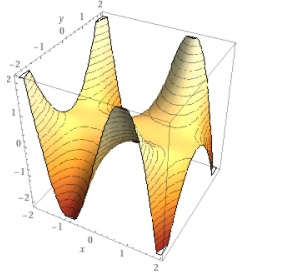
\includegraphics[width=.15\textwidth]{Dateien/07/07Konturplot.PNG}
 \vspace{-15pt}
\end{wrapfigure}
Betrachte $g:\mathbb{R}^2\to\mathbb{R},\,(x,y)\mapsto xy^2\cos(x)$.\\
Jeder Koordinate $(x,y)\in\mathbb{R}^2$ wird ein Wert in $\mathbb{R}$ (hier die $z$-Achse) zugeordnet, sodass man sich die Funktion als Teppich vorstellen kann.\\
Gerade bei solchen Funktionen ist der Anstieg in eine beliebige Richtung $v\in\mathbb{R}^2\setminus\MengeDirekt{0}$ interessant.
\end{Beispiel}

\begin{Def}
{Differenzierbarkeit in eine Richtung}
Wir nennen $f:U\to\mathbb{R}$ in $\xvec\in U$ \red{in Richtung} $\vvec\in U$ \red{differenzierbar}, wenn $\Tilde{f}:(-\epsilon,\epsilon)\to\mathbb{R}$ mit $\Tilde{f}(t)=f(\xvec+t\vvec)$ in $t=0$ differenzierbar ist.\\
Anschaulich machen wir also kleine Änderungen von $f$ in $\vvec$-Richtung und schauen, wie stark diese sind.
\end{Def}
\begin{Def}
{Richtungsableitung}
Wir nennen $(\partial_\vvec f)(\xvec)=\diff{}{t}\big|_{t=0}g(\xvec+t\vvec)=\Tilde{f}'(0)$ die \red{Ableitung von $f$ in Richtung $\vvec$.}
\end{Def}
\begin{Beispiel}
{Richtungsableitung}
Sei $\vvec=\MatrixInline{1\\1}$, so ist für $g=xy^2\cos(x)$ aus dem obigen Beispiel
\begin{equation*}
    g(\xvec+t\vvec)=g\BracedIn{\MatrixInline{x+t\\y+t}}=\BracedIn{x+t}\BracedIn{y+t}^2\cos(x+t).
\end{equation*}
Somit ist die Ableitung in $\vvec$-Richtung
\begin{align*}
    (\partial_\vvec g)(\xvec)&=\diff{}{t}\big|_{t=0}g(\xvec+t\vvec)\\
    &=\BracedInSqr{(y+t)^2\cos(x+t)+2(x+t)(y+t)\cos(x+t)-(x+t)(y+t)^2\sin(x+t)}_{t=0}\\
    &=(y^2+2xy)\cos(x)-xy^2\sin^2(x).
\end{align*}
\end{Beispiel}
\blue{Später lernt ihr noch eine weitere Möglichkeit mithilfe des Gradienten kennen, um sowas zu berechnen.}
\begin{Satz}
{Rechenregeln}{Regeln für Richtungsableitungen}
Für $f,g:\mathbb{R}^n\to\mathbb{R}$, die jeweils in $\xvec\in\mathbb{R}^n$ in Richtung $\vvec\in\mathbb{R}^n$ differenzierbar sind, gelten die üblichen Rechenregeln:
\begin{enumerate}
    \item \textbf{Linearität}:
    \begin{equation*}
        \boxed{\partial_\vvec(\lambda f+\mu g)(\xvec)=\lambda \partial_\vvec f(\xvec)+\mu\partial_\vvec  g(\xvec)}.
    \end{equation*}
    \item \textbf{Produktregel}:
    \begin{equation*}
        \boxed{\partial_\vvec (fg)(\xvec)=\partial_\vvec f(\xvec)g(\xvec)+f(\xvec)\partial_\vvec g(\xvec)}.
    \end{equation*}
    \item \textbf{Quotientenregel}:\\
    Ist $g(\xvec)\neq 0$, so gilt
    \begin{equation*}
        \boxed{\partial_\vvec \BracedIn{\frac{f}{g}}(\xvec)=\frac{\partial_\vvec f(\xvec)g(\xvec)-f(\xvec)\partial_\vvec g(\xvec)}{g(\xvec)^2}}.
    \end{equation*}
\end{enumerate}
\end{Satz}
\subsubsection{Partielle Ableitungen}
\blue{Die Mühe mit den Richtungsableitungen müssen wir uns aber nicht immer machen. Meistens reicht es, die Änderung der Funktion in Richtung der Koordinatenachsen zu betrachten.}
\begin{Def}
{Partielle Ableitung}
Wenn $f$ in $\xvec\in U$ in alle Koordinatenrichtungen differenzierbar ist, nennen wir $f$ in $\xvec$ \red{partiell differenzierbar} und\footnote{wobei $i$ die Koordinatenrichtungen des $\mathbb{R}^n$ sind} $(\partial_if)(\xvec)$ die $i$-te \red{partielle Ableitung} in $\xvec$.\\
\blue{\textbf{Notation}:\\
Wir schreiben dann $\partial_i f$ oder $\diffp{f}{x_i}$.}
\end{Def}
\blue{Die Ableitung in eine Koordinatenrichtung lässt sich einfach ausführen, indem die anderen Koordinaten konstant gehalten werden.}
\begin{Beispiel}
{Partielle Ableitung}
Für die obige Funktion $g(x,y)=xy^2\cos(x)$ sind die partiellen Ableitungen
\begin{align*}
    \diffp{g(x,y)}{x}&=\partial_x(xy^2\cos(x))=y^2\cos(x) -xy^2\sin(x)\\
    \partial_y g(x,y)&=2xy\cos(x).
\end{align*}
\end{Beispiel}

\begin{Satz}
{Satz}{Partielle Differenzierbarkeit $\nRightarrow$ Stetigkeit}
Wie ihr im \Skript{} auf Folie 208 seht, impliziert partielle Differenzierbarkeit \underline{nicht} die Stetigkeit!
\end{Satz}
\begin{Def}
{Höhere Ableitungen und stetige Differenzierbarkeit}
Wie auch schon in 1D definieren wir höhere Ableitungen $\partial_i^{(k)}$ rekursiv.\\
Ist die k-te Ableitung $\frac{\partial^k f}{\partial x_1\partial x_2\ldots}$ stetig, so nennen wir $f$ \red{$k$-fach stetig differenzierbar}. 
\end{Def}
\blue{So weit, so gut. Was passiert aber, wenn wir in verschiedene Richtungen ableiten?\\
Tatsächlich ist hier die Reihenfolge nicht wichtig:}
\begin{Satz}
{Lemma}{Lemma von Schwarz}
Ist $f:U\to\mathbb{R}$ zweimal stetig differenzierbar, gilt für alle Koordinatenrichtungen $i,j\in\MengeDirekt{1,\ldots,n}$:
\begin{equation}
    \diffp{}{x_i}\BracedIn{\diffp{}{x_j}f}(\xvec)=\diffp{}{x_j}\BracedIn{\diffp{}{x_i}f}(\xvec)\quad\tx{bzw. }\partial_{x_i}\partial_{x_j}f=\partial_{x_j}\partial_{x_i}f.
\end{equation}
\end{Satz}
Dieser Satz ist enorm wichtig!
\begin{Beispiel}
{Zweite Ableitung}
Für die obige Funktion $g=xy^2\cos(x)$ haben wir
\begin{align*}
    \partial_x\partial_y g(x,y)&=\partial_x(2xy\cos(x))=2y\cos(x)-2xy\sin(x)\\
    \partial_y\partial_x g(x,y)&=\partial_y(y^2\cos(x)-xy^2\sin(x))=2y\cos(x)-2xy\sin(x).
\end{align*}
\end{Beispiel}

\begin{Def}
{Gradient}
Den $n\times 1$-Vektor $\grad f=\MatrixInline{\partial_{x_1}f\\\vdots\\\partial_{x_n}f}$, der zeilenweise die partiellen Ableitungen von $f$ enthält, nennen wir \red{Gradienten} von $f$.
\end{Def}
\begin{Beispiel}
{Gradient einer Funktion}
Für die obige Funktion $g=xy^2\cos(x)$ ist
\begin{equation*}
    \grad f=\Matrix{\partial_x f\\\partial_y f}=\Matrix{y^2\cos(x)-xy^2\sin(x)\\2xy\cos(x)}.
\end{equation*}
\end{Beispiel}
\begin{Def}
{Vektorfeld}
Der Gradient ist das erste Beispiel für ein \red{Vektorfeld}, weil $\grad f:\mathbb{R}^n\to\mathbb{R}^n$.
\end{Def}
\blue{Anschaulich ordnen Vektorfelder jedem Punkt des Urbildraumes einen Vektor zu, der im Falle eines Gradienten in die Richtung des größten Anstiegs der Funktion $f$ zeigt.\\
Daher gilt in der Physik für konservative Kraftfelder auch, dass die Kraft sich aus einem skalaren Potential mittels $\Fvec=-\grad V$ gewinnen lässt, d. h., dass die Kraft immer entgegen der Richtung des höchsten Potentialanstiegs zeigt.}
\begin{Satz}
{Satz}{Produktregel für den Gradienten}
Für zwei Funktionen $f,g:U\to \mathbb{R}$ gilt: $\grad(f g)=g\grad f+f\grad g$.
\end{Satz}
\begin{Beispiel}
{Wichtiges Beispiel für rotationssymmetrische Funktionen}
Ist $r(\xvec)=\Norm{\xvec}=\sqrt{x_1^2+x_2^2+x_3^2}$ der Abstand vom Ursprung und $f:\mathbb{R}_+\to\mathbb{R} $ eine differenzierbare Funktion, die nur von $r$ abhängt, so ist also $F(\xvec)=f(r(\xvec))$ für alle $\xvec\in\mathbb{R}^3\setminus\MengeDirekt{0}$ partiell differenzierbar und es gilt mit der Kettenregel
\begin{align*}
    \partial_iF(\xvec)&=\partial_i(f(r(\xvec)))=f'(r(\xvec))\partial_ir(\xvec)\\
    &=f'(r)\partial_i\sqrt{x_1^2+x_2^2+x_3^2}=f'(r)\frac{2x_i}{2\sqrt{x_1^2+x_2^2+x_3^2}}=\frac{x_i}{r}f'(r),
\end{align*}
sodass für den Gradienten gilt
\begin{equation*}
    \grad F(\xvec)=\frac{f'(r)}{r}\Matrix{x_1\\x_2\\x_3}.
\end{equation*}
Als Beispiel betrachten wir die Funktion $F:\mathbb{R}^2\to\mathbb{R},\, F(\xvec)=e^{\sqrt{x^2+y^2}^3}=e^{r^3}$.\\
Hier haben wir
\begin{equation*}
    \grad (e^{r(\xvec)})=(e^{r^3})'\frac{1}{r}\Matrix{x\\y}=\frac{3r^2}{r}e^{r^3}\Matrix{x\\y}=3\sqrt{x^2+y^2}e^{\sqrt{x^2+y^2}^3}\Matrix{x\\y}.
\end{equation*}
\end{Beispiel}

\begin{Def}
{Divergenz}
Wir nennen ein Vektorfeld $F:\mathbb{R}^n\to\mathbb{R}^n$ partiell differenzierbar, wenn jede Komponentenfunktion partiell differenzierbar ist.\\
Die Abbildung $\divv:\mathbb{R}^n\to\mathbb{R},\,F(\xvec)\to\divv(F(\xvec))=\sum_{i=1}^n\partial_iF_i(\xvec)$ nennen wir \red{Divergenz} von $F$.
\end{Def}
\begin{Beispiel}
{Anschauung zur Divergenz}
\begin{itemize}
    \item Betrachte $F:\mathbb{R}^2\to\mathbb{R}^2,\,F(x,y)=\MatrixInline{-y\\x}$, so ist $\divv F=\partial_x(-y)+\partial_y(x)=0$.
    \item Betrachte $F:\mathbb{R}^2\to\mathbb{R}^2,\,F(x,y)=\MatrixInline{x\\y}$, so ist $\divv F=2$.
\end{itemize}
    \begin{center}
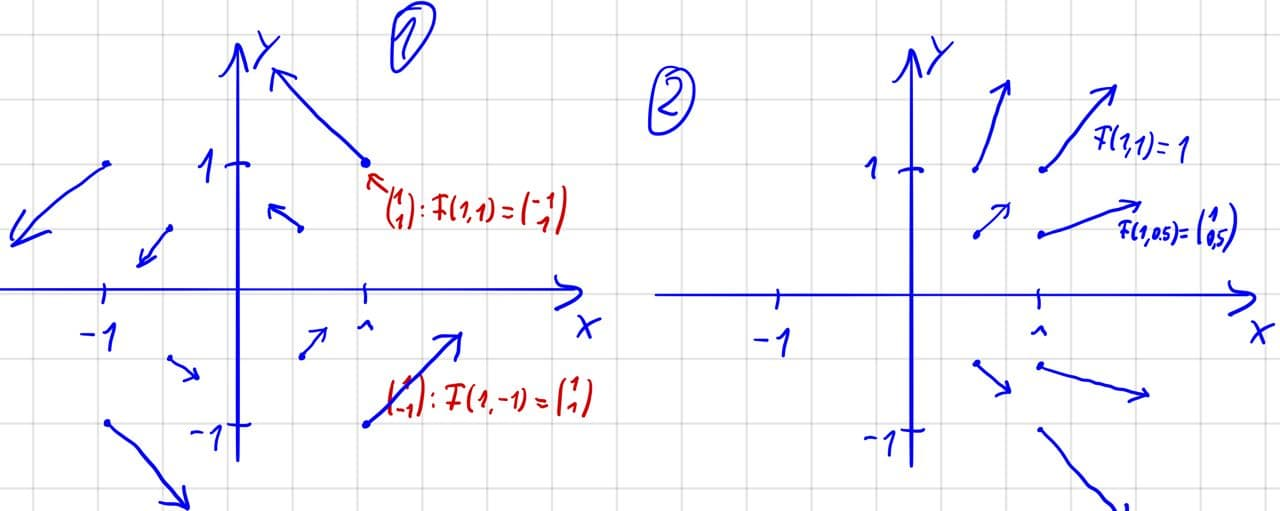
\includegraphics[width=.35\textwidth]{Dateien/07/07Vektorfelder.jpg}
    \end{center}
\blue{Die Divergenz im Punkt $\xvec$ sagt uns, wie stark die Vektoren des Vektorfelds dort \textit{auseinanderdriften}.}
\end{Beispiel}
\begin{Satz}
{Satz}{Leibnizregel für Divergenz}
Für ein in $\xvec$ differenzierbares Vektorfeld $\vvec:U\to\mathbb{R}^n$ und in $\xvec$ differenzierbare Funktion $f:U\to \mathbb{R}$ ist $f\cdot \vvec$ in $\xvec$ differenzierbar und es gilt
\begin{equation}
    \divv (f\vvec)(\xvec)=\BiFo{\grad f(\xvec),\vvec(\xvec)}+f(\xvec)\divv\vvec(\xvec),
\end{equation}
wobei $\BiFoLeer$ das kanonische Skalarprodukt sei.
\end{Satz}

\begin{Def}
{Laplace-Operator}
Für zweimal partiell differenzierbare Funktionen $f:U\to\mathbb{R}$ definieren wir den \red{Laplace-Operator} $\Delta f:U\to \mathbb{R}$ als
\begin{equation*}
    \Delta f:=\divv \grad f=\sum_{i=1}^n\partial_i^2f.
\end{equation*}
\end{Def}
\begin{Satz}
{Satz}{Die dritte Produktregel heute}
Für zweifach partiell differenzierbare Funktionen $f,g:U\to\mathbb{R}$ gilt:
\begin{equation*}
    \Delta (f g)=f\Delta g+g\Delta f+2\BiFo{\grad f,\grad g}.
\end{equation*}
\end{Satz}
\begin{Def}
{Vektorprodukt}
Im $\mathbb{R}^3$ definieren wir die schiefsymmetrische\footnote{$\vvec\times\Vec{w}=-\Vec{w}\times \vvec$} bilineare Abbildung $\times$ als das \red{Vektorprodukt}:
\begin{equation*}
    \times:\mathbb{R}^3\times \mathbb{R}^3\to\mathbb{R}^3,\,(\xvec,\yvec)\mapsto \xvec\times\yvec:=\Matrix{x_2y_3-x_3y_2\\x_3y_1-x_1y_3\\x_1y_2-x_2y_1}.
\end{equation*}
\end{Def}
\blue{\textbf{Merkhilfe}:\\
Dafür könnt ihr euch entweder die obersten Indizes merken und dann sehen, dass diese nach unten gehend immer um 1 erhöht werden, also $2\to3, 3\to1$ etc., oder das so aufmalen:
\begin{center}
    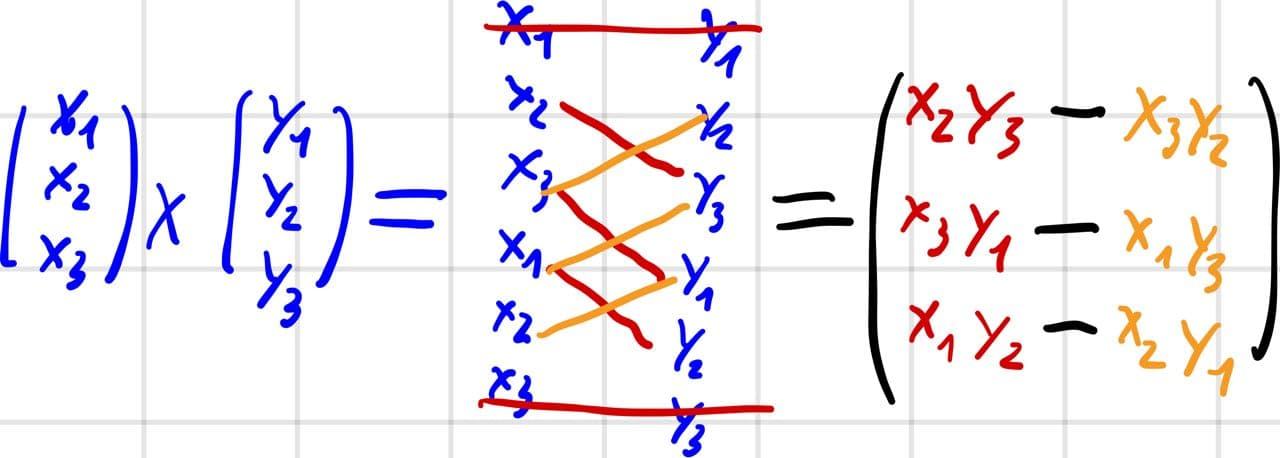
\includegraphics[width=.45\textwidth]{Dateien/07/07Vektorprodukt.jpg}
\end{center}}
\begin{Satz}
{Satz}{Eigenschaften des Vektorfeldes}
Die folgenden Eigenschaften für den $\mathbb{R}^3$ mit der durch die geordnete Basis gegebenen Orientierung habt ihr im \Skript{} festgehalten und auf euren Übungsblättern für alle $\xvec,\yvec\in\mathbb{R}^3$ gezeigt:
\begin{enumerate}
    \item $\xvec\times \yvec=-\yvec\times \xvec$.
    \item $\xvec\times\yvec$ ist senkrecht zu $\xvec$ und zu $\yvec$.
    \item $\Norm{\xvec\times\yvec}^2=\Norm{\xvec}^2\Norm{\yvec}^2-\BiFo{\xvec,\yvec}^2$.
    \item $\Norm{\xvec\times \yvec}=\Norm{\xvec}\Norm{\yvec}\sin\varphi$, wenn $\xvec,\yvec\in\mathbb{R}^3\setminus\MengeDirekt{0}$ und $\varphi=\angle(\xvec,\yvec)\in[0,\pi]$.
    \item $\xvec\times\yvec=0\iff (\xvec,\yvec)$ sind linear abhängig.\\
    Sind $(\xvec,\yvec)$ linear unabhängig, so ist $(\xvec,\yvec,(\xvec\times\yvec))$ eine positiv orientierte Basis.
    \item Sind $\xvec$ und $\yvec$ orthonormal, so ist $(\xvec,\yvec,(\xvec\times\yvec))$ eine positiv orientierte Orthonormalbasis.
\end{enumerate}
\end{Satz}
\begin{Beispiel}
{Geometrische Diskussion}
In der analytischen Geometrie habt ihr schon mit Vektoren aus dem $\mathbb{R}^3$ hantiert. Hier noch einmal die wichtigsten Erkenntnisse mit Veranschaulichungen (siehe unten) zu Vektoren in 2D:
\begin{enumerate}
    \item \textbf{Addition}:\\
    Die Summe zweier Vektoren kann man als \textit{aneinanderhängen} auffassen.
    \item \textbf{Subtraktion}:\\
    Die Strecke zwischen zwei Punkten $A$ und $B$ ist $\Vec{AB}=\Vec{b}-\Vec{a}$.
    \item \textbf{Skalare Multiplikation}:\\
    Für $\lambda\in\mathbb{R}$, $\vvec\in\mathbb{R}^3$ ändert die Multiplikation $\lambda\vvec$ anschaulich die Länge des Vektors.
    \item \textbf{Geradengleichung}:\\
    Punkte $\xvec$ auf einer Geraden können wir daher als Summe aus einem Stützvektor $\Vec{s}$ und einem skaliertem Vektor $\Vec{r}$ aufschreiben:
    \begin{equation*}
        \xvec=\Vec{s}+t\Vec{r}.
    \end{equation*}
    \item \textbf{Skalarprodukt}:\\
    Das Skalarprodukt projiziert Vektoren aufeinander.
    \begin{equation*}
    \Vec{a}\cdot\Vec{b}:=\BiFo{\Vec{a},\Vec{b}}=\Norm{\Vec{a}}\Norm{\Vec{b}}\cos\alpha\quad\tx{und }\Vec{a}\perp\Vec{b}\iff \Vec{a}\cdot\Vec{b}=0.
    \end{equation*}
    \item \textbf{Vektorprodukt}:\\
    Das Vektorprodukt bildet einen positiv (rechtshändig) orientierten Vektor $\Vec{n}=\Vec{a}\times \Vec{b}$ aus den Vektoren $\Vec{a}$ und $\Vec{b}$, der die Länge $\Norm{\nvec}=\Norm{\avec\times\bvec}=\Norm{a}\Norm{b}\sin\alpha$ hat, welche der Fläche des von $\avec$ und $\bvec$ aufgespannten Parallelogramms entspricht.
    \item \textbf{Ebenengleichung}:\\
    Wie bei der Geradengleichung können wir alle Punkte $\xvec$ auf einer Ebene durch die Summe aus einem Stützvektor $\svec$ und zwei (linear unabhängigen) Richtungsvektoren $\rvec_1$ und $\rvec_2$ beschreiben:
    \begin{equation*}
         E=\Menge{\xvec\in\mathbb{R}}{\xvec=\svec+t\rvec_1+s\rvec_2}=\svec+\Spann{\rvec_1,\rvec_2}.
    \end{equation*}
    Diese ist ein zweidimensionaler, affiner\footnote{d. h. um einen Vektor vom Ursprung verschobener} Untervektorraum des $\mathbb{R}^3$.
    \item \textbf{Hessesche Normalform}:
    Eine weitere Beschreibung einer Ebene bietet sich, wenn man aus den Richtungsvektoren $\rvec_1$ und $\rvec_2$ einen normierten Normalenvektor $\nvec:=\frac{\rvec_1\times\rvec_2}{\Norm{\rvec_1\times\rvec_2}}$ konstruiert, der senkrecht zur Ebene steht.\\
    Falls $\xvec\in E$, so ist die Verbindungsstrecke von $\svec$ zu $\xvec$ daher senkrecht zu $\nvec$, also $(\xvec-\svec)\cdot \nvec=0$.\\
    Formt man dies um, so ergibt sich $(\xvec-\svec)\cdot \nvec=0\iff \xvec\nvec=\svec\nvec$.\\
    Also ist eine äquivalente Beschreibung von $E$ gegeben durch
    \begin{equation*}
        E=\Menge{\xvec\in\mathbb{R}^3}{\xvec\cdot \nvec=w},
    \end{equation*}
    wobei $\nvec:=\frac{\rvec_1\times\rvec_2}{\Norm{\rvec_1\times\rvec_2}}$ und der Skalar $w=\nvec\cdot\svec\in\mathbb{R}$ sind.
\end{enumerate}
\begin{center}
    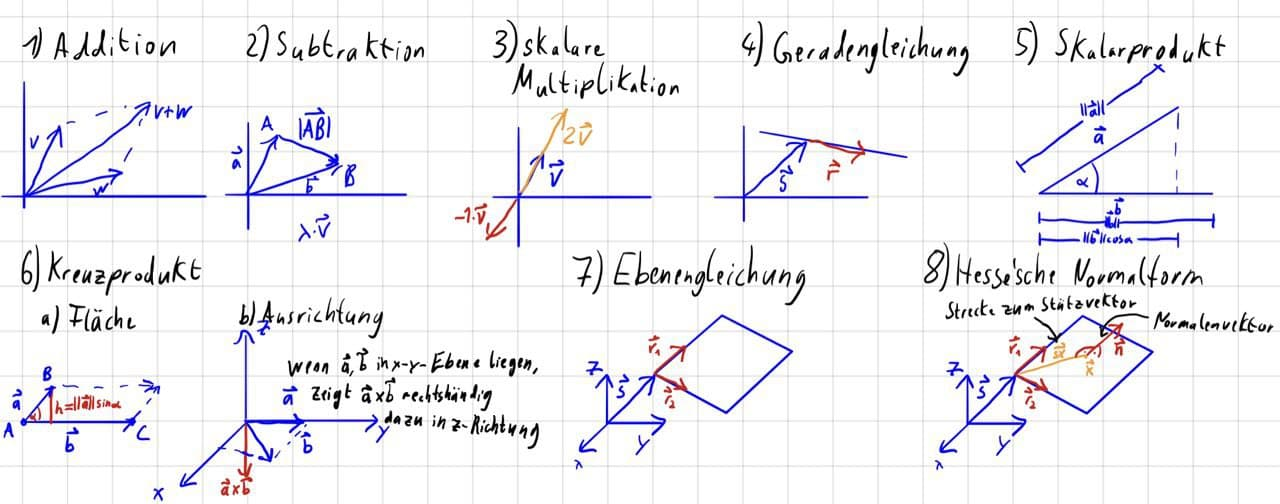
\includegraphics[width=.9\textwidth]{Dateien/07/07Vektoranschauungen.jpg}
\end{center}
\end{Beispiel}
\begin{Def}
{Spatprodukt}
\begin{wrapfigure}{r}[0pt]{.35\textwidth}
 \vspace{-15pt}
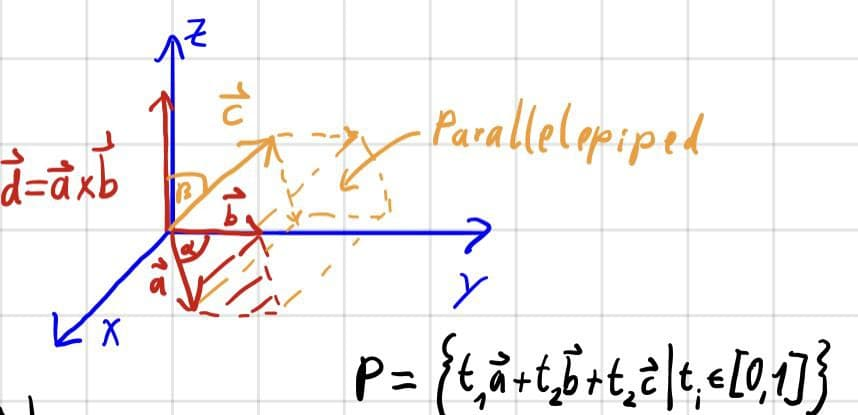
\includegraphics[width=.35\textwidth]{Dateien/07/07Parallelepiped.jpg}
 \vspace{-15pt}
\end{wrapfigure}
Zusätzlich gibt es noch das \red{Spatprodukt} aus drei Vektoren $\avec,\bvec,\cvec\in\mathbb{R}^3$, welches das \underline{orientierte} Volumen des von $\avec$, $\bvec$ und $\cvec$ aufgespannten Parallelepipeds beschreibt.\\
Dieses ist durch die Kombination von Kreuz- und Skalarprodukt gegeben:
\begin{equation}
    V:\mathbb{R}^3\times\mathbb{R}^3\times\mathbb{R}^3\to\mathbb{R},\, (\avec,\bvec,\cvec)\mapsto\BiFo{\avec\times\bvec,\cvec}=\det\Matrix{\avec &\bvec &\cvec}
\end{equation}
Die Gleichheit im letzten Schritt ist ein Satz. Hier haben wir also eine anschauliche Bedeutung der Determinante.
\end{Def}
\begin{Def}
{Rotation}
Mithilfe des Vektorproduktes können wir nun durch $\rot:\mathbb{R}^3\to\mathbb{R}^3$ eine weitere Abbildung für Vektorfelder $\Fvec:\mathbb{R}^3\to\mathbb{R}^3$ definieren:
\begin{equation}
    \rot \Fvec:=\Matrix{\partial_2 F_3-\partial_3 F_2\\\partial_3 F_1-\partial_1 F_3\\\partial_1 F_2-\partial_2 F_1}=\nablavec\times \Fvec,
\end{equation}
wobei wir $\nablavec:=\MatrixInline{\partial_1\\\partial_2\\\partial_3}$ als Abkürzung gewählt haben.
\end{Def}
\begin{Beispiel}
{Rotation}
\begin{wrapfigure}{r}[0pt]{.25\textwidth}
 \vspace{-15pt}
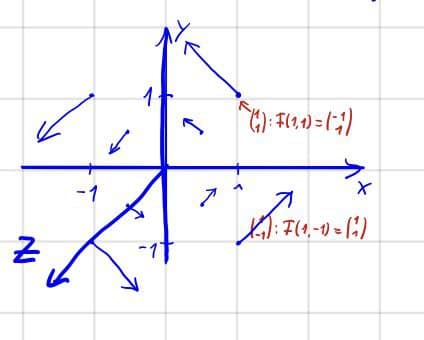
\includegraphics[width=.25\textwidth]{Dateien/07/07Rotation.jpg}
 \vspace{-15pt}
\end{wrapfigure}
Für die oben schon betrachtete, auf $\mathbb{R}^3$ erweiterte Abbildung $\Fvec:\mathbb{R}^3\to\mathbb{R}^3,\,\Fvec(x,y,z)=\MatrixInline{-y\\x\\0}$ ergibt sich $\rot \Fvec=\MatrixInline{\partial_y 0-\partial_zx\\\partial_z (-y)-\partial_x 0\\\partial_x x-\partial_y (-y)}=\MatrixInline{0\\0\\2}$.\\
Unabhängig davon, wo wir uns befinden, rotiert das Feld um die $z$-Achse entgegen\footnote{also mathematisch positiv} des Uhrzeigersinnes.
\end{Beispiel}

\begin{Satz}
{Satz}{Doppelanwendung}
Aufgrund der Vertauschbarkeit partieller Ableitungen gilt für zweimal stetig differenzierbare Abbildungen $\Fvec:U\to\mathbb{R}^3$ und $f:U\to\mathbb{R}$ 
\begin{equation}
    \rot\grad f=0\quad \tx{und} \quad \grad \divv \Fvec=\Vec{0}.
\end{equation}
\end{Satz}
\blue{Wenden wir die Rotation auf ein Kraftfeld $\Fvec$ an und ist $\rot\Fvec=0$, so können wir folgern, dass $\Fvec$ konservativ ist und gemäß $\Fvec=-\grad V$ einem Potential $V:\mathbb{R}^3\to\mathbb{R}$ entstammt. Dies ist häufig sehr nützlich!}

\subsection{Differenzierbare Abbildungen}
\blue{Jetzt wird es ein bisschen komplizierter, also gut aufpassen und vor allem immer genau auf die Dimensionen der Räume achten, zwischen denen wir abbilden!}\\
\red{Warum brauchen wir überhaupt noch einen weiteren Begriff der Differenzierbarkeit?}\\
\blue{Das Problem an den partiellen Ableitungen ist, dass diese die Funktionen für's Ableiten auf eine Variable reduzieren und z. B. auch unstetige Funktionen partiell differenzierbar sein können (vgl. Folie 208).\\
Außerdem haben wir bisher nur Funktionen betrachtet,, die vom $\mathbb{R}^n$ nach $\mathbb{R}$ abbilden.\\
Im Folgenden werden Abbildungen behandelt, die allgemein vom $\mathbb{R}^n\to\mathbb{R}^m$ abbilden!\\
Hier ist die Differenzierbarkeit zu sehen als 'was passiert im Bildraum, d. h. wie stark ändert sich die Funktion in die Koordinatenrichtungen, wenn wir uns im Urbildraum in eine bestimmte Richtung bewegen?'}
\subsubsection{Motivation}
Zum Einstieg erinnern wir uns zurück an einen Satz aus MfP1 (Folien 234 - 236):
\begin{Wiederholung}
{Affine Approximation}
\begin{wrapfigure}{r}[0pt]{.23\textwidth}
 \vspace{-15pt}
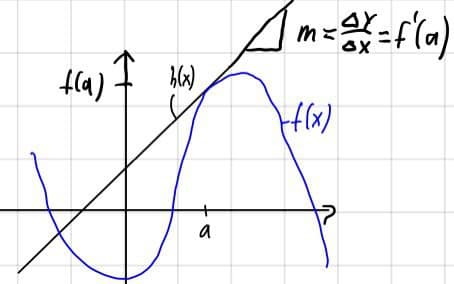
\includegraphics[width=.23\textwidth]{Dateien/07/07Tangentengleichung.jpg}
 \vspace{-15pt}
\end{wrapfigure}
Die \red{affine Approximation} einer Funktion $f$ im Punkt $a\in D$ ist als 
\begin{equation}
    h:D\to\mathbb{R}, \,\boxed{h(x)=f(a)+f'(a)(x-a)}
\end{equation}
definiert.
\end{Wiederholung}
$h(x)$ entspricht der \underline{Tangentengleichung}, die ihr vielleicht noch aus unseren MfP1-Notizen oder der Schule kennt.\\
Unter Umständen ist es nützlich, diese Funktion als Annäherung zu $f(x)$ zu nutzen.\\
In diesem Fall kann man über das sogenannte \red{Restglied} $R(x)$ den Fehler dier Approximation abschätzen, es ist 
\begin{equation*}
    R(x)=f(x)-h(x)=f(x)-f'(a)(x-a)-f(a)
\end{equation*}
Außerdem entspricht diese Herangehensweise um $x=a$, die nach dem linearen Term abgebrochen wird.\\
In Bezug darauf hatten wir folgenden Satz gesehen:
\begin{Wiederholung}
{Differenzierbarkeit und affine Approximation}
Ist $f$ differenzierbar in $a\in D$, so gilt
\begin{equation*}
    \lim_{x\to a}\frac{f(x)-h(x)}{x-a}=0.
\end{equation*}
Falls $f$ stetig ist gilt andersherum:\\
Existiert $h(x)=c(x-a)+d$ (mit $c,d\in\mathbb{R}, \,a\in D$), sodass 
\begin{equation*}
    \lim_{x\to a}\frac{f(x)-h(x)}{x-a}=0
\end{equation*}
ist, so ist $f$ differenzierbar in $a$.\\
\Zb{Die erste Aussage ist leicht zu zeigen, denn mit der so definierten Funktion haben wir einfach
\begin{equation*}
    \frac{f(x)-h(x)}{x-a}=\frac{f(x)-f(a)}{x-a}-f'(a)\overset{x\to a}{\to}0.
\end{equation*}}
\end{Wiederholung}
Die affine Approximation ist also quasi nur eine andere Beschreibung der Ableitung. Wir werden gleich etwas kennenlernen, das $f'(a)$ in dieser Beschreibungsart gleicht.\\
Wir betrachten also anders aufgeschrieben
\begin{equation*}
    \lim_{x\to a}\frac{f(x)-f(a)-c(x-a)}{x-a}=0,
\end{equation*}
wobei wir sagen, dass dieses $c=f'(a)$ ist, wenn der Grenzwert existiert.\\
Setzen wir nun $x:=a+\xi$ bzw. $a=x-\xi$, so ergibt sich die Gleichung
\begin{equation*}
    \lim_{\xi\to0}\frac{f(a+\xi)-f(a)-c\xi}{\xi}=0,
\end{equation*}
eine Existenz dieses Grenzwertes mit einer geeigneten Konstanten $c$ ist also gleichbedeutend mit Differenzierbarkeit.\\
\blue{Für unsere allgemeine Definition auf höheren Räumen gehen wir nun ähnlich vor, allerdings tauschen wir $f(x)$ mit dem Vektor $\Fvec(\xvec)$, wobei $\Fvec:\mathbb{R}^n\to\mathbb{R}^m$ ist. Also muss auch $\xivec\in\mathbb{R}^n$ aus dem Urbildraum sein, d. h. statt der Konstanten $c$ benötigen wir eine\footnote{wie wir sehen werden lineare} Abbildung $A:\mathbb{R}^n\to\mathbb{R}^m$, die aus $\xivec$ einen Vektor aus $\mathbb{R}^m$ macht.}
\subsubsection{Verallgemeinerte Definition der Differenzierbarkeit}
\begin{Def}
{Totale Differenzierbarkeit}
Ist $U\subseteq\mathbb{R}^n$ offen und $\Fvec:U\to\mathbb{R}^m$ eine vektorwertige Abbildung, so heißt $\Fvec$ im Punkt $\xvec\in U$ \red{total differenzierbar}, falls eine \underline{lineare Abbildung} $A:\mathbb{R}^n\to\mathbb{R}^m$ existiert, sodass
\begin{equation}
    \lim_{\xivec\in\mathbb{R}^n\setminus\MengeDirekt{\Vec{0}},\xivec\to\Vec{0}}\frac{\Norm{\Fvec(\xvec-\xivec)-\Fvec(\xvec)-A(\xivec)}}{\Norm{\xivec}}=0
\end{equation}
ist. \blue{Zusätzlich benötigen wir also auch noch die Norm, um aus den ganzen Vektoren reelle Zahlen zu machen, für die wir sinnvoll Grenzwerte definiert haben.}\\
Wie gewohnt nennen wir $\Fvec:U\to\mathbb{R}^m$ \red{differenzierbar}, wenn $\Fvec$ differenzierbar für alle $\xvec\in U$ ist.
\end{Def}
\blue{Also nochmal:\\
Statt der linearen Funktion $A:\mathbb{R}\to\mathbb{R},\,\xi\mapsto c\xi$, die wir in der Motivation als Ableitung genutzt hatten, betrachten wir nun eine lineare Abbildung $A:\mathbb{R}^n\to\mathbb{R}^m,\,\xivec\to A(\xivec)$ und lassen statt der Zahl $\xi$ den Vektor $\xivec\in\mathbb{R}^n$ unter der Norm des $\mathbb{R}^n$ gegen 0 gehen.}
\begin{Def}
{Differential}
Die hierbei auftretende lineare Abbildung $A:\mathbb{R}^n\to\mathbb{R}^m$ ist \underline{eindeutig} und wird \red{Differential} von $\Fvec$ im Punkt $\xvec$ getauft.\\
Man schreibt auch
\begin{equation}
    d\Fvec_\xvec:=A:\mathbb{R}^n\to\mathbb{R}^m.
\end{equation}
\end{Def}
\blue{Als lineare Abbildung hat $d\Fvec_\xvec$ natürlich eine darstellende $m\times n$-Matrix. Diese hat folgende Berechnungsvorschrift:}
\begin{Satz}{Satz}
{Jacobi-Matrix{,} totale Differenzierbarkeit impliziert partielle}
Ist $\Fvec:\mathbb{R}^n\to\mathbb{R}^m$ in $\xvec$ total differenzierbar, so existiert für alle Richtungen $\vvec\in\mathbb{R}^n\setminus\MengeDirekt{\Vec{0}}$ und alle Komponenten $F_j(\xvec),\,j\in\MengeDirekt{1,\ldots,m}$ die Richtungsableitung mit\\
$\partial_\vvec(F_j(\xvec))=((d\Fvec_\xvec)_j(\vvec))$.\\
Die darstellende $m\times n$ Matrix $J_\xvec$ von $d\Fvec_\xvec$ ist dann gegeben durch
\begin{equation}
    J_\xvec=\Matrix{\partial_{x_1}F_1(\xvec)&\cdots&\partial_{x_n}F_1(\xvec)\\
    \vdots &\ddots& \vdots\\
    \partial_{x_1}F_m(\xvec)&\cdots&\partial_{x_n}F_m(\xvec)}=\Matrix{\grad(F_1(\xvec))^T\\\vdots\\\grad(F_m(\xvec))^T}.
\end{equation}
\end{Satz}

\begin{Beispiel}
{Anschauung der Jacobimatrix}
Wir betrachten wieder die obige Funktion $g:\mathbb{R}^2\to\mathbb{R},\,g(x,y)=xy^2\cos(x)$.\\
Das Differential wäre hier also auch eine lineare Abbildung $dg:\mathbb{R}^2\to\mathbb{R}$.\\
Im Punkt $\pvec\in\mathbb{R}^2$ ist $g(x,y)$ differenzierbar, wenn wir diesen anschaulich mit einer Tangentialebene approximieren können (analog zur Tangentengleichung für $f:\mathbb{R}\to\mathbb{R}$).\\
Die Jacobi-Matrix ist in diesem Beispiel die $(1\times2)$-Matrix
\begin{equation*}
    J_\xvec=\Matrix{\grad(g)^T}=\Matrix{\partial_xg(x,y)&\partial_yg(x,y)}=\Matrix{y^2(\cos(x)-x\sin(x))&2xy\cos(x)}.
\end{equation*}
\textbf{Gleichung der Tangentialebene}:\\
Nun wollen wir als Beispiel einmal die affine Approximation im Punkt $\pvec\in\mathbb{R}^2$ bestimmen, die (analog zu $h(x)=f(a)+f'(a)(x-a)$) folgende Form hat:
\begin{equation*}
    H(\xvec)=g(\pvec)+J_\pvec\cdot(\xvec-\pvec).
\end{equation*}
Als konkrete Beispiele betrachten wir die Punkte $\pvec_1=\MatrixInline{0\\1}$ und $\pvec_2=\Matrix{\pi\\-1}$:\\
Hier ist
\begin{align*}
    J_{\pvec_1}&=J_{(0,1)}=\Matrix{1(\cos(0)+0)&0}=\Matrix{1&0}\quad\tx{und}\quad g(0,1)=0\cdot1^2\cos(0)=0\\
    J_{\pvec_2}&=J_{(\pi,-1)}=\Matrix{-1&2\pi}\quad\tx{und}\quad g(\pi,-1)=\pi\cdot(-1)^2\cos(\pi)=-1.
\end{align*}
In drei Dimensionen entspricht $H(\xvec)$ dem $z$-Wert der Ebene, also haben wir
\begin{align*}
    z&=H(x,y)=g(0,1)+J_{(0,1)}\BracedIn{\Matrix{x\\y}-\Matrix{0\\1}}=0+\Matrix{1&0}\Matrix{x\\y-1}=x\\
    &\quad\implies x-z=0\\
    z&=H(x,y)=g(\pi,-1)+\Matrix{-1&2\pi}\Matrix{x-\pi\\y+1}=-\pi-x+\pi+2\pi y+2\pi\\
    &\quad\implies x-2\pi y+z=2\pi.
\end{align*}
Diese Ebenengleichungen können wir uns nun analog zu den Tangentengleichungen vorstellen.
\begin{center}
    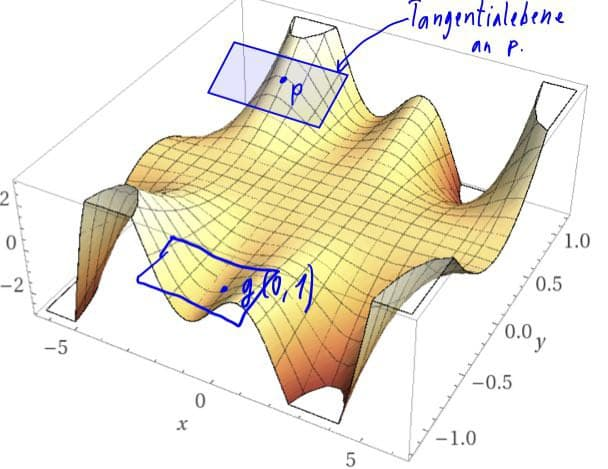
\includegraphics[width=.45\textwidth]{Dateien/07/07Tangentialebenen.jpg}
\end{center}
\end{Beispiel}
\subsubsection{Abschließende Sätze zur totalen Differenzierbarkeit}
Für die folgenden Sätze definieren wir  die offene Teilmenge $U\subseteq \mathbb{R}^n$.
\begin{Satz}
{Satz}{Jacobi-Matrix und Richtungsableitung}
Die Richtungsableitung $\partial_\vvec f$ einer Abbildung $f:U\to\mathbb{R}$ existiert $\forall \vvec\in U\setminus\MengeDirekt{\Vec{0}}$, wenn $f$ total differenzierbar ist.\\
Es gilt:
\begin{equation}
    \partial_\vvec f(\xvec)=df_\xvec(\vvec)=J_\xvec\vvec=\BiFo{\grad(f),\vvec}.
\end{equation}
\end{Satz}
\begin{Satz}
{Satz}{Totale Differenzierbarkeit impliziert Stetigkeit}
Ist $\Fvec:U\to\mathbb{R}^m$ in $\xvec\in U$ total differenzierbar, so ist $\Fvec$ stetig in $\xvec$.
\end{Satz}
Der folgende \red{wichtige} Satz gibt uns ein gutes Kriterium für die totale Differenzierbarkeit an die Hand:
\begin{Satz}
{Satz}{Zur totalen Differenzierbarkeit}
Falls $\Fvec:U\to\mathbb{R}^m$, wobei $\Fvec(\xvec)=\sum_{k=1}^mF_k(\xvec)\hat{\evec}_k$ \underline{partiell} differenzierbar ist und zusätzlich alle partiellen Ableitungen $\partial_iF_k$ in $\xvec\in U$ \underline{stetig} sind, ist $\Fvec$ in $\xvec$ total differenzierbar.
\end{Satz}
\blue{Da in der Jacobi-Matrix alle partiellen Ableitungen vorkommen, ist also $\Fvec$ total differenzierbar, sobald alle Komponenten der Jacobi-Matrix stetig sind.}
\begin{Beispiel}
{Zur totalen Differenzierbarkeit}
Sei $\Fvec:\mathbb{R}^2\to\mathbb{R}^3,\,(x,y)\mapsto\MatrixInline{y\sin(x)\\4y\\e^{xy}}$. Hier haben wir
\begin{equation*}
    d\Fvec_{(x,y)}=\Matrix{\grad(F_1(x,y))^T\\\grad(F_2(x,y))^T\\\grad(F_3(x,y))^T}=\Matrix{\partial_x(y\sin(x))&\partial_y(y\sin(x))\\\partial_x(4y)&\partial_y(4y)\\\partial_x(e^{xy})&\partial_y(e^{xy})}=\Matrix{y\cos(x)&\sin(x)\\0&4\\ye^{xy}&xe^{xy}}.
\end{equation*}
Alle Komponenten sind stetig $\forall\xvec=(x,y)\in\mathbb{R}^2$.\\
Also ist $\Fvec$ total differenzierbar und somit insbesondere stetig.
\end{Beispiel}